\begin{figure}[htbp]
\section*{ IKZF1}
\centering
\begin{subfigure}[b]{0.95\textwidth}
\centering
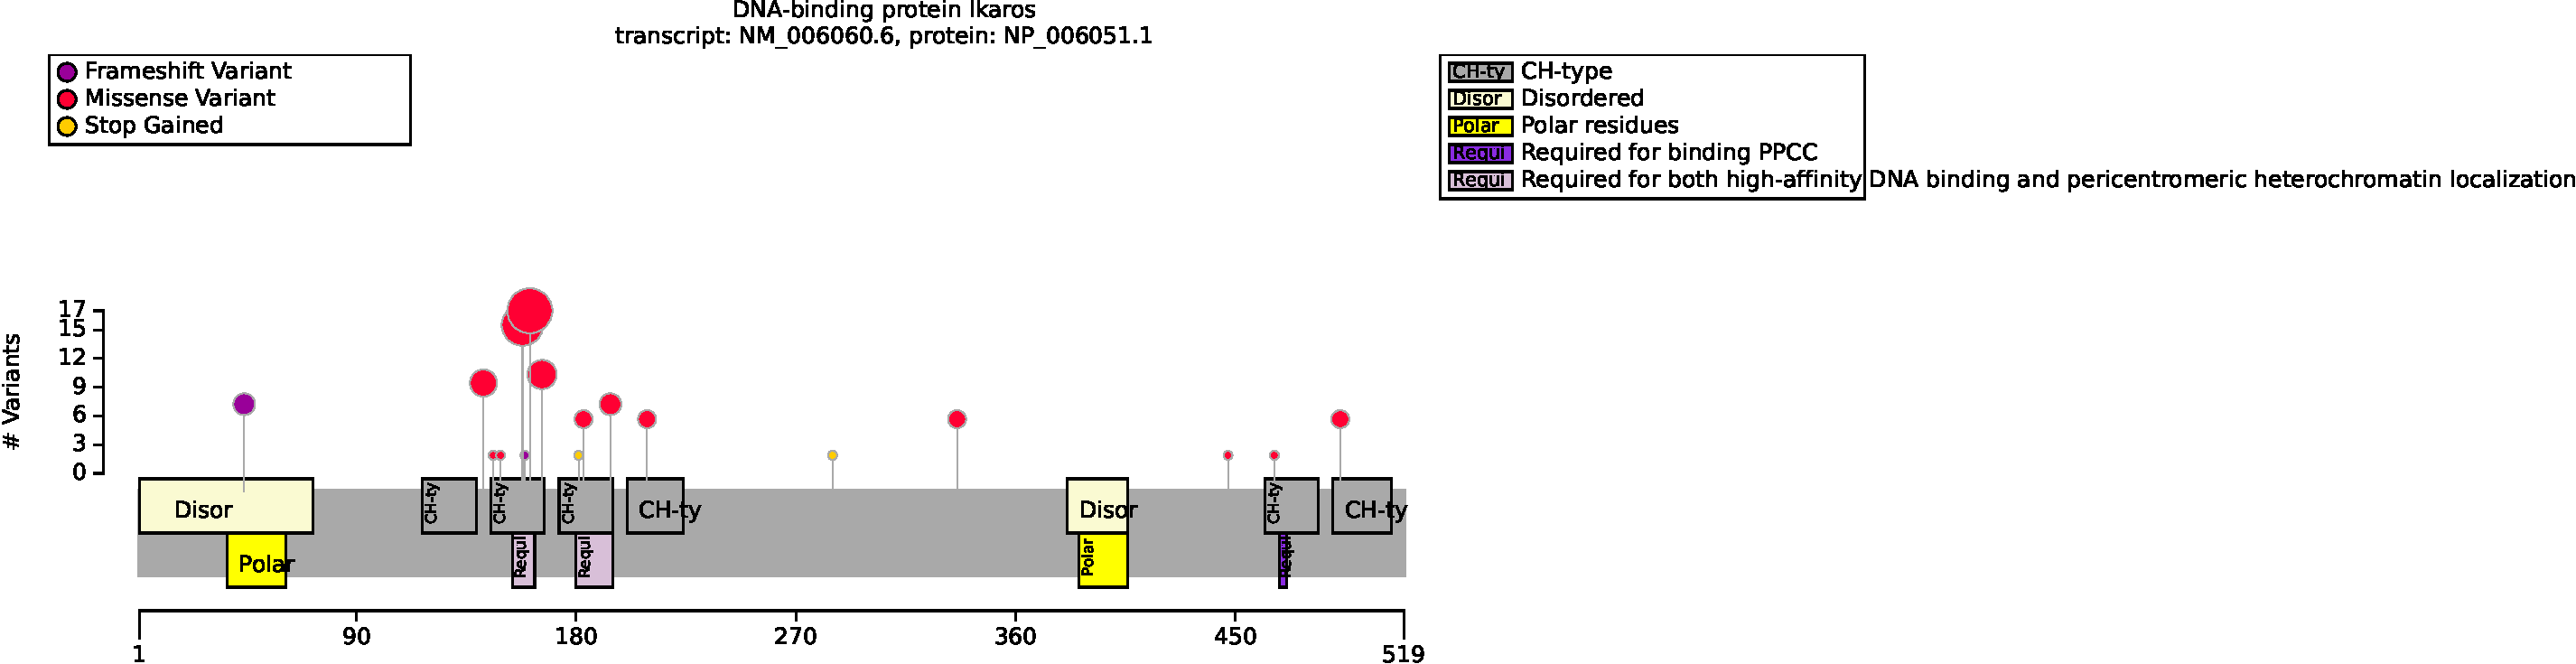
\includegraphics[width=\textwidth]{ img/IKZF1_protein_diagram.pdf} 
\captionsetup{justification=raggedright,singlelinecheck=false}
\caption{Distribution of variants in IKZF1}
\end{subfigure}

\vspace{2em}

\begin{subfigure}[b]{0.95\textwidth}
\centering
\resizebox{\textwidth}{!}{
\begin{tabular}{llllrr}
\toprule
HPO term & p.Asn159Ser & Other variant & p-value & adj. p-value\\
\midrule
Recurrent pneumonia [HP:0006532] & 7/9 (78\%) & 7/39 (18\%) & 0.001 & 0.035\\
T-cell acute lymphoblastic leukemias [HP:0006727] & 3/13 (23\%) & 0/69 (0\%) & 0.003 & 0.047\\
\bottomrule
\end{tabular}
}
\captionsetup{justification=raggedright,singlelinecheck=false}
\caption{         Fisher Exact Test performed to compare HPO annotation frequency with respect to p.Asn159Ser and Other variant. Total of
        29 tests were performed. }
\end{subfigure}
\vspace{2em}
\begin{subfigure}[b]{0.95\textwidth}
\centering
\resizebox{\textwidth}{!}{
\begin{tabular}{llllrr}
\toprule
Genotype (A) & Genotype (B) & total tests performed & significant results\\
\midrule
Missense & oher & 34 & 0\\
\bottomrule
\end{tabular}
}
\captionsetup{justification=raggedright,singlelinecheck=false}
\caption{Fisher Exact Test performed to compare HPO annotation frequency with respect to genotypes. }
\end{subfigure}

\vspace{2em}

\caption{ The cohort comprised 82 individuals (34 females, 37 males, 11 with unknown sex). 5 of these individuals were reported to be deceased. 
A total of 66 HPO terms were used to annotate the cohort. Disease diagnosis: Immunodeficiency, common variable, 13 (OMIM:616873). 
The variant p.Asn159Ser was functionally characterized to be dominant-negative and result in a combined-immunodeficiency phenotype that 
was distinct from other IKZF1 variants \cite{PMID_29889099}. A total of 26 unique variant alleles were found in \textit{IKZF1} (transcript: \texttt{NM\_006060.6}, protein id: \texttt{NP\_006051.1}).}
\end{figure}
